\documentclass[conference]{IEEEtran}
\usepackage{cite}
\usepackage{amsmath,amssymb,amsfonts}
\usepackage{algorithmic}
\usepackage{graphicx}
\usepackage{dirtytalk}
\usepackage{textcomp}
\usepackage{xcolor}
% \def\BibTeX{{\rm B\kern-.05em{\sc i\kern-.025em b}\kern-.08em
%     T\kern-.1667em\lower.7ex\hbox{E}\kern-.125emX}}


% Using BibTex, with specified choices of what to include in bibliography
\usepackage[backend=bibtex,
sorting=none, % sort entries by appearance
isbn=true, % include isbn, doi, url etc or not in bibliography entry
doi=false,
url=false,
maxnames=1,
eprint=false,
abbreviate=true,
style=ieee]{biblatex}

% adding the bibliography file
\addbibresource{references}


\begin{document}

\title{Quantum Error Correction: Surface Codes}

\author{
  \IEEEauthorblockN{Asier Galicia}
  \IEEEauthorblockA{\textit{Faculty of Applied Physics} \\
  \textit{Delft University of Technology}\\
    Delft, Netherlands \\
    A.Galiciamartinez@student.tudelft.nl}

  \and

  \IEEEauthorblockN{Nicholas Zutt}
  \IEEEauthorblockA{\textit{Faculty of Applied Physics} \\
  \textit{Delft University of Technology}\\
Delft, Netherlands \\
N.C.F.Zutt@student.tudelft.nl}
}

\maketitle


\begin{abstract}
Quantum error correction (QEC) schemes make possible the reliable use of quantum computers in
tackling computationally difficult problems. In order to be useful, encoded
qubits and quantum operations have to be implemented in a fault-tolerant way. We
present an overview of quantum error correction and fault-tolerance, followed by
a more in depth review of a particular, promising error-correction scheme: the
surface code. We include a brief discussion of error decoding algorithms and a
review of recent experimental implementations of surface codes.
\end{abstract}

\begin{IEEEkeywords}
  quantum computation, error correction, surface code, error decoding, fault-tolerance
\end{IEEEkeywords}

\section{Introduction}
Quantum computers are devices that exploit the features of quantum mechanics at
the smallest scales of reality. They even have the potential to solve
computational problems that are not feasible for conventional computers
\cite{nielsen_chuang_2010}. Some of the most famous applications are the
accurate simulation of physics \cite{feynman82_simul_physic_with_comput}, fast
database searching provided by Grover's algorithm \cite{Grover_1996} and the
polynomial time solution for factoring large composite numbers, provided by
Shor's algorithm \cite{Shor_1997}, which has far-reaching consequences for
current methods in cryptography. However, there are still key technological
challenges that need to be overcome before this technology can be realized.

To date, superconducting LC circuits have shown the greatest promise in forming
effective quantum bits (or qubits) \cite{Rol_2019}
\cite{barends14_super_quant_circuit_at_surfac}, however several other platforms,
such as quantum dots \cite{huang19_fidel_bench_two_qubit_gates_silic}
\cite{Lawrie_2020}, NV-centres in diamond \cite{Taminiau_2014}, and even
topological qubits in semi-conducting nanowires \cite{Mourik_2012}, have seen
growing interest and recent development. Nevertheless, they all suffer from some
form of noise, of a slightly different nature in each case, which poses
major challenges in the realization of a scalable quantum computer.

Accounting for this noise is undoubtedly a daunting task. For that, different
approaches have been developed which are usually grouped as part of
\textit{quantum error suppression} (QES), such as dynamical decoupling, which
attempt to reduce the noise at the hardware level, and \textit{quantum error
  correction} (QEC) techniques, which aim to correct errors once they have
occurred. In particular, the latter approach has undergone rapid development in
recent decades from the schemes proposed by Shor \cite{Shor_1995_QEC} and Steane
\cite{Steane_1996_QEC} to the new promising \textit{surface codes}
\cite{fowler12_surfac_codes} that have higher tolerance to errors and require
fewer interactions among the qubits.

In this article, we review the key principles of quantum error correction,
discuss ...

\subsection{Principles of Quantum Error Correction}
% I think that here we should mention what the [[n,k,d]] code is.
In the basic theory of quantum error correction, quantum states are encoded into
several physical qubits. By performing the appropriate parity checks, it is
possible to probe the state of the encoded qubit (which is comprised of many
physical qubits) without changing its state, in order to detect errors on
individual physical qubits. These parity checks are the \textit{stabilizers} of
the error correction code; when all stabilizer measurements return an eigenvalue
of $+1$, it signals that no error has occurred \cite{nielsen_chuang_2010}.
Effective encoding protocols are such that each error process gives rise to a
unique syndrome, which is just the list of stabilizer measurement outcomes,
which provides the information needed to correct the error \cite{fowler12_surfac_codes}.

\begin{figure}
  \centering
  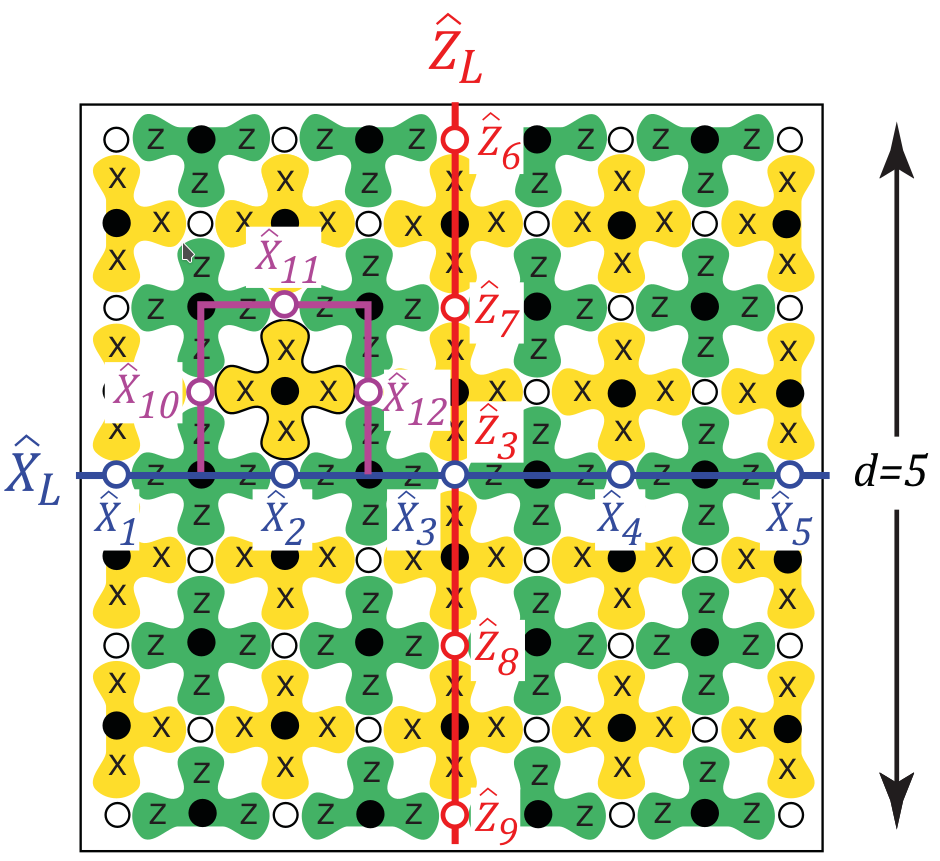
\includegraphics[width=0.4\textwidth]{images/surface_code.png}
  \caption{A 2D array of qubits implementing the surface code. Data qubits are
    the white circles, which are connected to 2 $Z$- and 2 $X$-stabilizers
    respectively. This code is capable of precisely characterizing Pauli noise
    due to the complimentary spacing of the $X$ and $Z$ checks. Figure from
    \cite{fowler12_surfac_codes}.}
  \label{fig:surface_code}
\end{figure}

In any real implementation of physical qubits, there are several sources of
error. State preparation and measurement may not be carried out perfectly.
Coherent errors also occur through the imperfect application of quantum gates in
circuits \cite{Devitt_2013}. Error models and error correction schemes are all
predicated on the assumption that low-weight errors (affecting only a few
qubits) are more likely than high weight errors. In other words, error
probabilities must be small \cite{terhal15}. In principle though, all these
(small) sources of error can be corrected for using a variety of encoding and
detection schemes.

The error detection scheme implemented by the surface code, shown in Fig.
\ref{fig:surface_code}, is capable of precisely identifying errors in large
arrays of qubits. The $X$- and $Z$-stabilizer ancillas conduct parity
measurements between the data qubits to which they are connected through a
sequence of CNOT operations. Should an error occur on a given data qubit,
depending on the error type ($X$, $Y$, or $Z$) either the $X$ or $Z$ (or both)
type stabilizers will fire (return an outcome of $-1$ in their measurement),
alerting us to the error.

One great strength of the surface code is its ability to diagnose multiple
errors simultaneously. Should two adjacent $X$-checks fire at one end of the
surface, while two $Z$-checks fire at the other end, we can conclude that a
phase-flip error occurred on the data qubit between the two $X$-checks, while a
bit-flip error occurred between the $Z$-checks. One must be careful, however,
because decoding the error syndrome for any code is a problem without a unique
solution \cite{terhal15}. Taking the top-left data qubit in Fig. \ref{fig:surface_code} as an
example, one can confirm that a bit-flip error on that qubit would give rise to
the exact same syndrome as a series of bit-flip errors on the rest of the top
row of data qubits. For systems with small error probabilities, the single
bit-flip error is of course much more likely than the long series of errors
required to produce the same syndrome, but as the error rate grows, such
mistakes in identifying the cause of a syndrome become more commonplace. 

When a syndrome is misinterpreted, the code implements the \textit{wrong
  correction}, and this can lead to a logical level operation being applied to
the logical qubit. The rate at which this occurs, called the \textit{logical
  error rate}, as a function of the physical error rate of the code is of great
interest in characterizing the effectiveness of an error correction protocol.


%%% Local Variables:
%%% mode: latex
%%% TeX-master: "QEC_paper"
%%% End:


\section{Principles of quantum error correction}
%how physical implementations are affected by noise, how to mitigate this
%definition fault tolerance
As mentioned in the precious section, errors can occur at every point in the
execution of an algorithm. State preparation, measurement, and gate operations
are examples of operations that are affected by these errors. Furthermore, the
errors occurring at any of these steps may propagate through the different
operations to the rest of the components of the system. This could lead to
cascading errors throughout the entire process, destroying all reliability in
the computation through loss of coherence. If a quantum computer is ever to be
realized, errors must be carefully contained.

It is in this context of error propagation that the concept of
\textit{fault-tolerant} quantum computing arises. A certain operation is said to
be fault-tolerant if a single error occurring at any step between two QEC cycles
causes at most one error at each of the logical blocks involved in the operation
\cite{Devitt_2013}. An example of fault-tolerant operation is shown in Fig.
\ref{fig:fault_tol} (b) where a bit-flip error in the top logical block
propagates only once to the bottom logical block (in contrast to (a) where it
propagates multiply). It is noteworthy that the constraint of only one
error propagating to different logical blocks can be relaxed when increasing the
code distance \cite{Devitt_2013}. In fact, for $d$ distance codes, it suffices
to require $d-2$ errors at each logical block.

\begin{figure}[htbp]
  \centering
  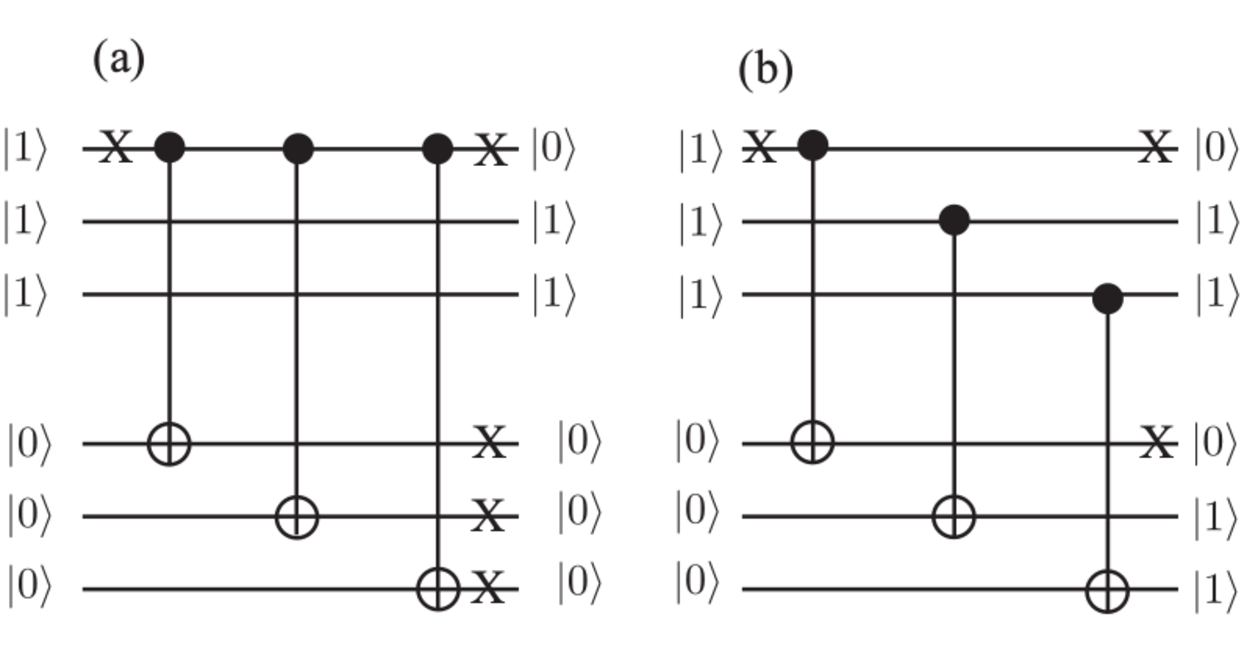
\includegraphics[width=0.5\textwidth]{images/fault_tolerance.pdf}
  \caption{Exmple of an operation that is not fault-tolerant (a) and one that is
    fault-tolerant (b). In these examples a bit-flip error in the top logical
    block propagates through the CNOT gates to the bottom logical block.}
  \label{fig:fault_tol}
\end{figure}

% Maybe logical error rates should be defined hered
However, it is not enough to have a fault tolerant set of operations in order to
implement a successful QEC protocol. Indeed, we want the logical error rate to
lower when increasing the code distance, either by means of concatenation or, in
the case of surface codes, by increasing the size of the surface. However, a high
error rate would prevent this from happening. In the case of surfaces codes, a
simple empirical equation that encapsulates the main properties of the logical
error rate obtained in simulations is
\cite{fowler12_surfac_codes}
\begin{equation}
  \label{eq:1}
  P_L = c\left(\frac{p}{p_{th}}\right)^{\frac{ d+1 }{2}},
\end{equation}
where d is the distance of the QEC protocol employed, $c$ is a constant that
depends on the exact characteristics of the error model, $p$ is the error rate
under sensible assumptions and $p_{th}$ is the error rate threshold. This
equation clearly shows the benefit of increasing the code distance, since for
$p<p_{th}$, the logical error rate decreases with increasing distance. Even
though these threshold error rates vary depending on the employed error model,
the current consensus puts the threshold at around $10^{-2}$ \cite{terhal15}
\cite{Versluis_2017}. However, it is yet to be shown experimentally a physical
system that accomplishes such low error rates.



%%% Local Variables:
%%% mode: latex
%%% TeX-master: "QEC_paper"
%%% End:


\section{Defect qubits in surface codes}
%encoding, detecting errors, ``correcting'' errors in software, fault tolerant
%operations?
%decoding algorithms
The discussion thus far has focused mainly on encoding logical states in the
entire 2D array of qubits that make up a particular surface. However, creating
different 2D sheets for each logical qubit is not the most effective way to
scale up this scheme for multiple logicals. One key candidate approach suggests
encoding qubits using \textit{defects} in the lattice structure of the surface
code, by switching off certain parity measurements to define logical qubits. We
will now outline this procedure.

In order to encode a qubit in a surface code, it suffices to define two logical
operations, namely $Z_L$ and $X_L$, which fulfill the commutation relation
$[Z_L,X_L] = 2Z_LX_L$. When multiple qubits are required, the $X_L$ and $Z_L$
operations among different qubits must commute. Figure \ref{fig:surface_code}
shows one of the possible set of physical operations that can lead to the
required logical operations. In this case, a chain of Z (X) gates in the data
qubits, represented with the red (blue) line, are one of the multiple choices to
define a logical $Z_L$ ($X_L$) operation.

\begin{figure}[htbp]
  \centering
  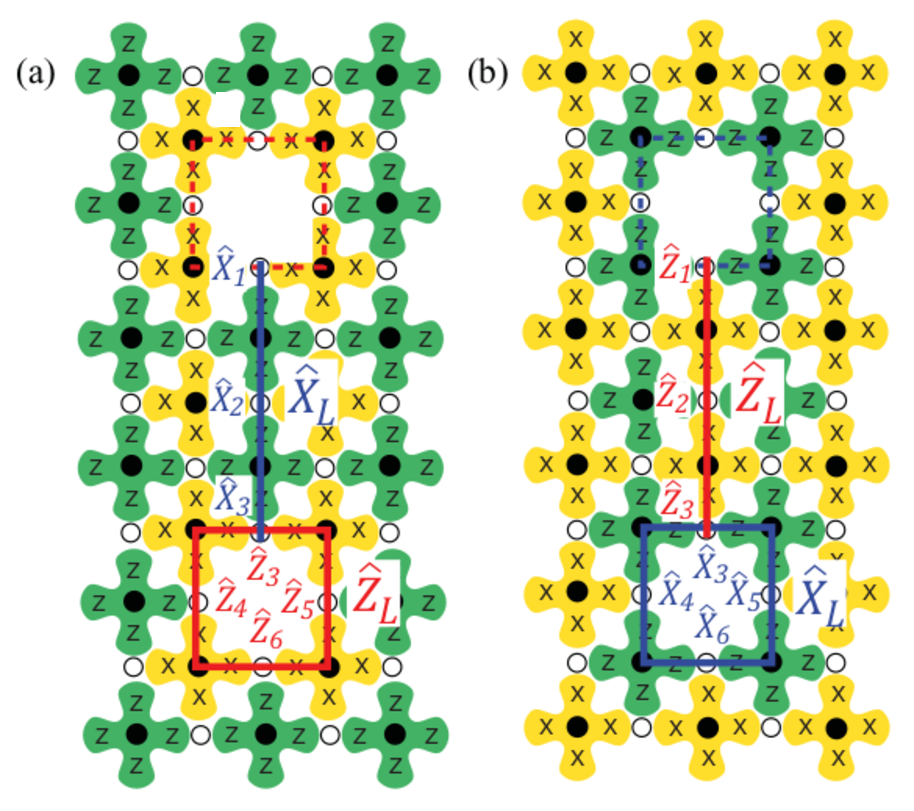
\includegraphics[width=0.5\textwidth]{images/surface_code_cuts.pdf}
  \caption{Examples of a Z-cut (a) and X-cut (b) qubit in a surface lattice. The
    logical gates are defined such that they satisfy the appropriate commutation
    relations. Moving defects further from each other can increase the code
    distance (the minimum number of gates required for a logical operation).}
  \label{fig:cuts}
\end{figure}

However, even though a set qubits may be fully defined in terms of these
operations, it is still necessary to perform arbitrary rotations and multi-qubit
gates on them. It is a well-known result of quantum computation that that it
suffices to be able to apply the standard H, T and CNOT gates to perform
universal computation \cite{nielsen_chuang_2010}. However, from the DiVincenzo
criteria \cite{DiCincenzoCriteria}, we see that initialization and
measurement capabilities are also necessary.

Although all these operations can be performed using one lattice per qubit,
it is more efficient to use a defect based approach. In this case, a qubit
consists of two Z-cut (X-cut) defects, where, in its simplest form, two Z (X)
stabilizers stop participating in the QEC cycle. Figure \ref{fig:cuts} shows an
example of both Z-cut and X-cut qubits. The figure also shows with blue
(red) line how to obtain $Z_L$ ($X_L$) operations using $Z$ ($X$) operations in
the data qubits.

These logical gates define the qubit but performing arbitrary operations on them
is highly non-trivial. Reviewing in full detail all the operations in these
defect based qubits is beyond the current scope, though there are several
techniques that are worth mentioning. The defects that make up the qubits on the
plane can be moved while preserving logical states, and a CNOT operation can be
can be performed by moving one of the defects of a Z-cut qubit around one of the
defects of an X-cut qubit. These \textit{braiding operations} are performed
ensuring fault tolerance since the qubits always maintain at least their initial
code distance. Furthermore, every measure explicitly performed on the data
qubits while moving the defects, can be checked with the surrounding stabilizers
to ensure fault tolerance.

The other technique worth outlining is the implementation of arbitrary
Z-rotations (making a T gate possible). This is performed in an indirect way by
first preparing an ancilla. Performing arbitrary rotations require the
preparation of an arbitrary state, which is by itself a challenging task. In
this case, the approach followed consists on starting with a two Z-cut qubit
separated by only one data where the arbitrary Z-rotation is easy to perform.
Afterwards, the Z-cuts are separated to protect the state for the
remainder of the operation. Due to the typically low fidelity of the prepared
ancilla, several such ancillas are prepared and undergo purification to create
one high fidelity ancilla for use. These techniques make clear how a universal
gate set can be implemented using the surface code.


%%% Local Variables:
%%% mode: latex
%%% TeX-master: "QEC_paper"
%%% End:


\section{Decoding algorithms}
% optimal decoding vs. efficient decoding
% minimum weight perfect matching
% maximum likelihood
Once the error syndrome is known, it is necessary to perform a decoding process
to obtain the best guess on what error occurred. The main challenges consist on
obtaining a fast yet precise algorithm, which is preferably scalable with the
number of data qubits. Regarding to the corrections, it should be noted that the
errors are bookeped using software based techniques in such a way that the
correction is applied at the end of the computation process by adapting the
measurement output of the data qubits.

We would like to mention two different approaches. The \textit{maximum
  likelihood method}\cite{} stands for applying the most probable correction. In
this case, a lookup table could be designed to speed up the process. However it
requires accurate error model. Furthermore, the lookup table approach becomes
impractical with increasing number data qubits due to the exponential increase
in possible syndromes. Another approach that is being considered is the
\textit{minimum weight perfect matching}\cite{} algorithm. In this case, error
syndromes are represented as a weighted graph. Afterwards, the vertices of this
graph are paired minimizing their total weight. This pairing establishes the
operation necessary to correct the error. This approach is shown to be robust
and it does not scale exponentially with the number of data qubits. Nevertheless
it is slower than using a lookup table.



% Finally, another approach that is being considered is to
% train an neural network in order to perform the decoding efficiently. This
% approach would be extremely time efficient but it would require large amounts of
% training data for increasing number of qubits. However, recent research shows
% that this may still be viable option \cite{}.


%%% Local Variables:
%%% mode: latex
%%% TeX-master: "QEC_paper"
%%% End:

\section{Experimental Implementations}
Implementing a full surface code capable of detecting and correcting a wide
range of possible errors requires at the very least, dozens of physical qubits
capable of performing high fidelity single and two-qubit gate operations. It
isn't surprising then that such a physical implementation remains out of reach.

Current practical limitations notwithstanding, significant progress has been
made recently in the effort to realize these codes experimentally. Recently,
Andersen \textit{et al.} have realized an experimental setup capable of
repeatedly detecting any single error \cite{Andersen_2020}. Their code is very
small, consisting of just four data qubits and three ancillas (1 $X$-check and 2
$Z$-checks) as shown in Fig. \ref{fig:seven_qbit_code}. Repeated ancilla
measurement was made possible through recent advancements in multi-plexing
readout of superconducting qubits (which were used in this case) which limit
cross-talk and allow for high-fidelity entangling operations and ancilla readout
\cite{barends14_super_quant_circuit_at_surfac} \cite{Bultink_2020}.

\begin{figure}[h]
  \centering
  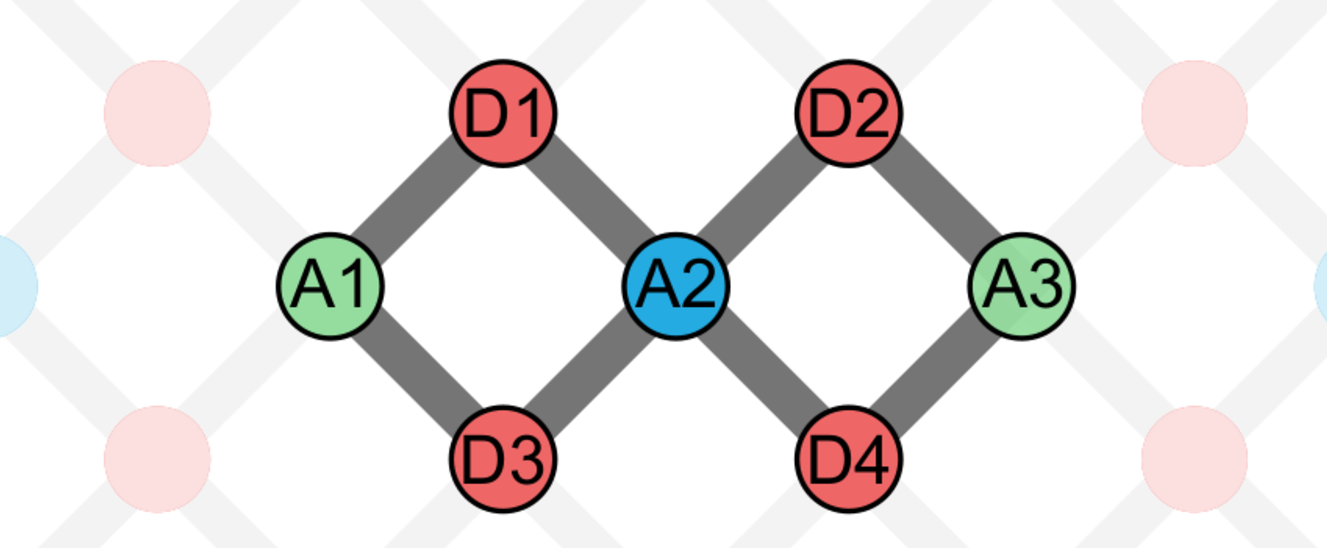
\includegraphics[width=0.4\textwidth]{images/seven_qbit_code.pdf}
  \caption{A seven qubit surface code, with four (red) data qubits, one (blue)
    X-type ancilla and 2 (green) Z-type ancilla qubits. This is the smallest
    instance of the surface code capable of detecting arbitrary single qubit
    errors. Figure from \cite{Andersen_2020}.}
  \label{fig:seven_qbit_code}
\end{figure}

%Talk about this paragraph
Surface codes are capable of successfully detecting $d-1$ errors, and correcting
up to $\lfloor{(d-1)/2} \rfloor$ errors, where $d$ is the code's distance.
Andersen \textit{et al.} define the logical qubit states
\begin{align}
|0\rangle_L &= \frac{1}{\sqrt{2}} (|0000\rangle + |1111\rangle) , \\
|1\rangle_L &= \frac{1}{\sqrt{2}} (|0101\rangle + |1010\rangle) 
\end{align}
from which it is easy to see that this code has distance $d=2$. It is therefore
capable of \textit{detecting} errors, but not of \textit{correcting} them. This
can be seen by realizing that, for example, an $X$-error on D2 or D4 give rise
to the exact same syndrome.

Remarkably, despite an inability to explicitly correct for detected errors,
Andersen \textit{et al.}, by measuring ancillas for errors, can ensure a longer
logical qubit lifetime than any of its physical constituents. By checking
repeatedly that no stabilizer measurement has fired, and discarding runs where
they do, they show that the decay of the expectation values $\langle Z_L
\rangle$ and $\langle X_L \rangle$ both exceed equivalent expectation values for
the best physical data qubit. The fact that repeated stabilizer measurement
outcomes that signal no error whatsoever are possible here, is a testament to the
precision with which superconducting qubits can be initialized, manipulated and
measured. As further research realizes qubits with error rates further and
further below the error threshold for reliable error correction, larger codes
and better stabilizer measurement can make large-scale, fault-tolerant
computation possible. Versluis \textit{et al.} have proposed a scheme for
scalable QEC using transmon superconducting qubits that focuses on developing an
eight-qubit unit cell that can be used to tile together a full surface code
\cite{Versluis_2017}.

Implementations of the surface code are not only limited to superconducting
qubits, either. Recent proposals, such as that of Hill \textit{et al.} , to
implement the surface code in silicon quantum dots promise to drastically reduce
the overhead per qubit by exploiting the uniformity between phosphorus donor
nuclear spin qubits \cite{silicon_surface_code}. Their proposal addresses the
requirement for repeated stabilizer measurement by implementing shared control
over all the qubits, resulting in a control architecture capable of executing
the full sequence of CNOT gates for all ancilla qubits in just four steps. The
number of steps required is independent of qubit number, which makes this
approach more easily scalable. Though the results presented by Hill \textit{et
  al.} are simulations, the authors stress that all the key requirements for
implementing this scheme in a physical system have already been individually
demonstrated.

%%% Local Variables:
%%% mode: latex
%%% TeX-master: "QEC_paper"
%%% End:


\section{Conclusion}
Quantum error correction, and its realization experimentally, remains a key
milestone in the development of a scalable, fault-tolerant quantum computer.
Progress in the development of high threshold error correcting codes, especially
the surface code, and the fault-tolerant application of quantum gates at the
logical level, provide a possible road-map to a truly universal quantum
computer.

Many challenges have yet to be addressed, though. Higher fidelity control and
measurement of qubits would certainly help is creating codes with physical error
rates below threshold, but scaling up to system sizes beyond that of just a
handful of qubits also necessitates the development of novel electrical control
architectures capable of issuing extremely accurate manipulation and read-out
instructions to a large number of qubits, while operating at cryogenic
temperatures.

A surface code comprised of 9 data qubits and 8 ancilla qubits, commonly called
the surface-17, is the smallest possible surface code capable of detecting and
correcting arbitrary single-qubit errors. The experimental implementation of
such a code, probing an increase in the fidelity of the logical quibt, would
constitute a great step forward in the realization of fault-tolerant QEC.


%%% Local Variables:
%%% mode: latex
%%% TeX-master: "QEC_paper"
%%% End:


\pagebreak
\printbibliography
\end{document}
